\chapter{Experimental Results}
\label{chapter6}
\thispagestyle{empty}

\begin{quotation}
{\footnotesize
\noindent\emph{``Quote 6''}
\begin{flushright}
Author 6
\end{flushright}
}
\end{quotation}

\vspace{0.5cm}

%\noindent Si mostra il progetto dal punto di vista sperimentale, le cose materialmente realizzate. In questa sezione si mostrano le attivit\`a sperimentali svolte, si illustra il funzionamento del sistema (a grandi linee) e si spiegano i risultati ottenuti con la loro valutazione critica. Bisogna introdurre dati sulla complessit\`a degli algoritmi e valutare l'efficienza del sistema.

\section{Accuracy of the Detection Algorithm}

\vspace{0.5cm}

\section{Accuracy of Humans}

\vspace{0.5cm}

\section{Accuracy of Algorithms}

(rif. paper)

\subsection{Performances of Algorithms on MITOS Dataset}
\label{ch6:icpr_perf}

We report here the performances of the best-scoring algorithms that participated to the ICPR2012 Contest, as shown on the contest website (Figure \ref{ch6:fig3}).
The principal metric adopted to compare algorithms is the $F_1$-Score (Figure \ref{ch6:fig3:a}) , but also precision and recall are shown \ref{ch6:fig3:b}. 

\begin{figure}[!htb]
  \centering
    \subfigure[F-Score]{
      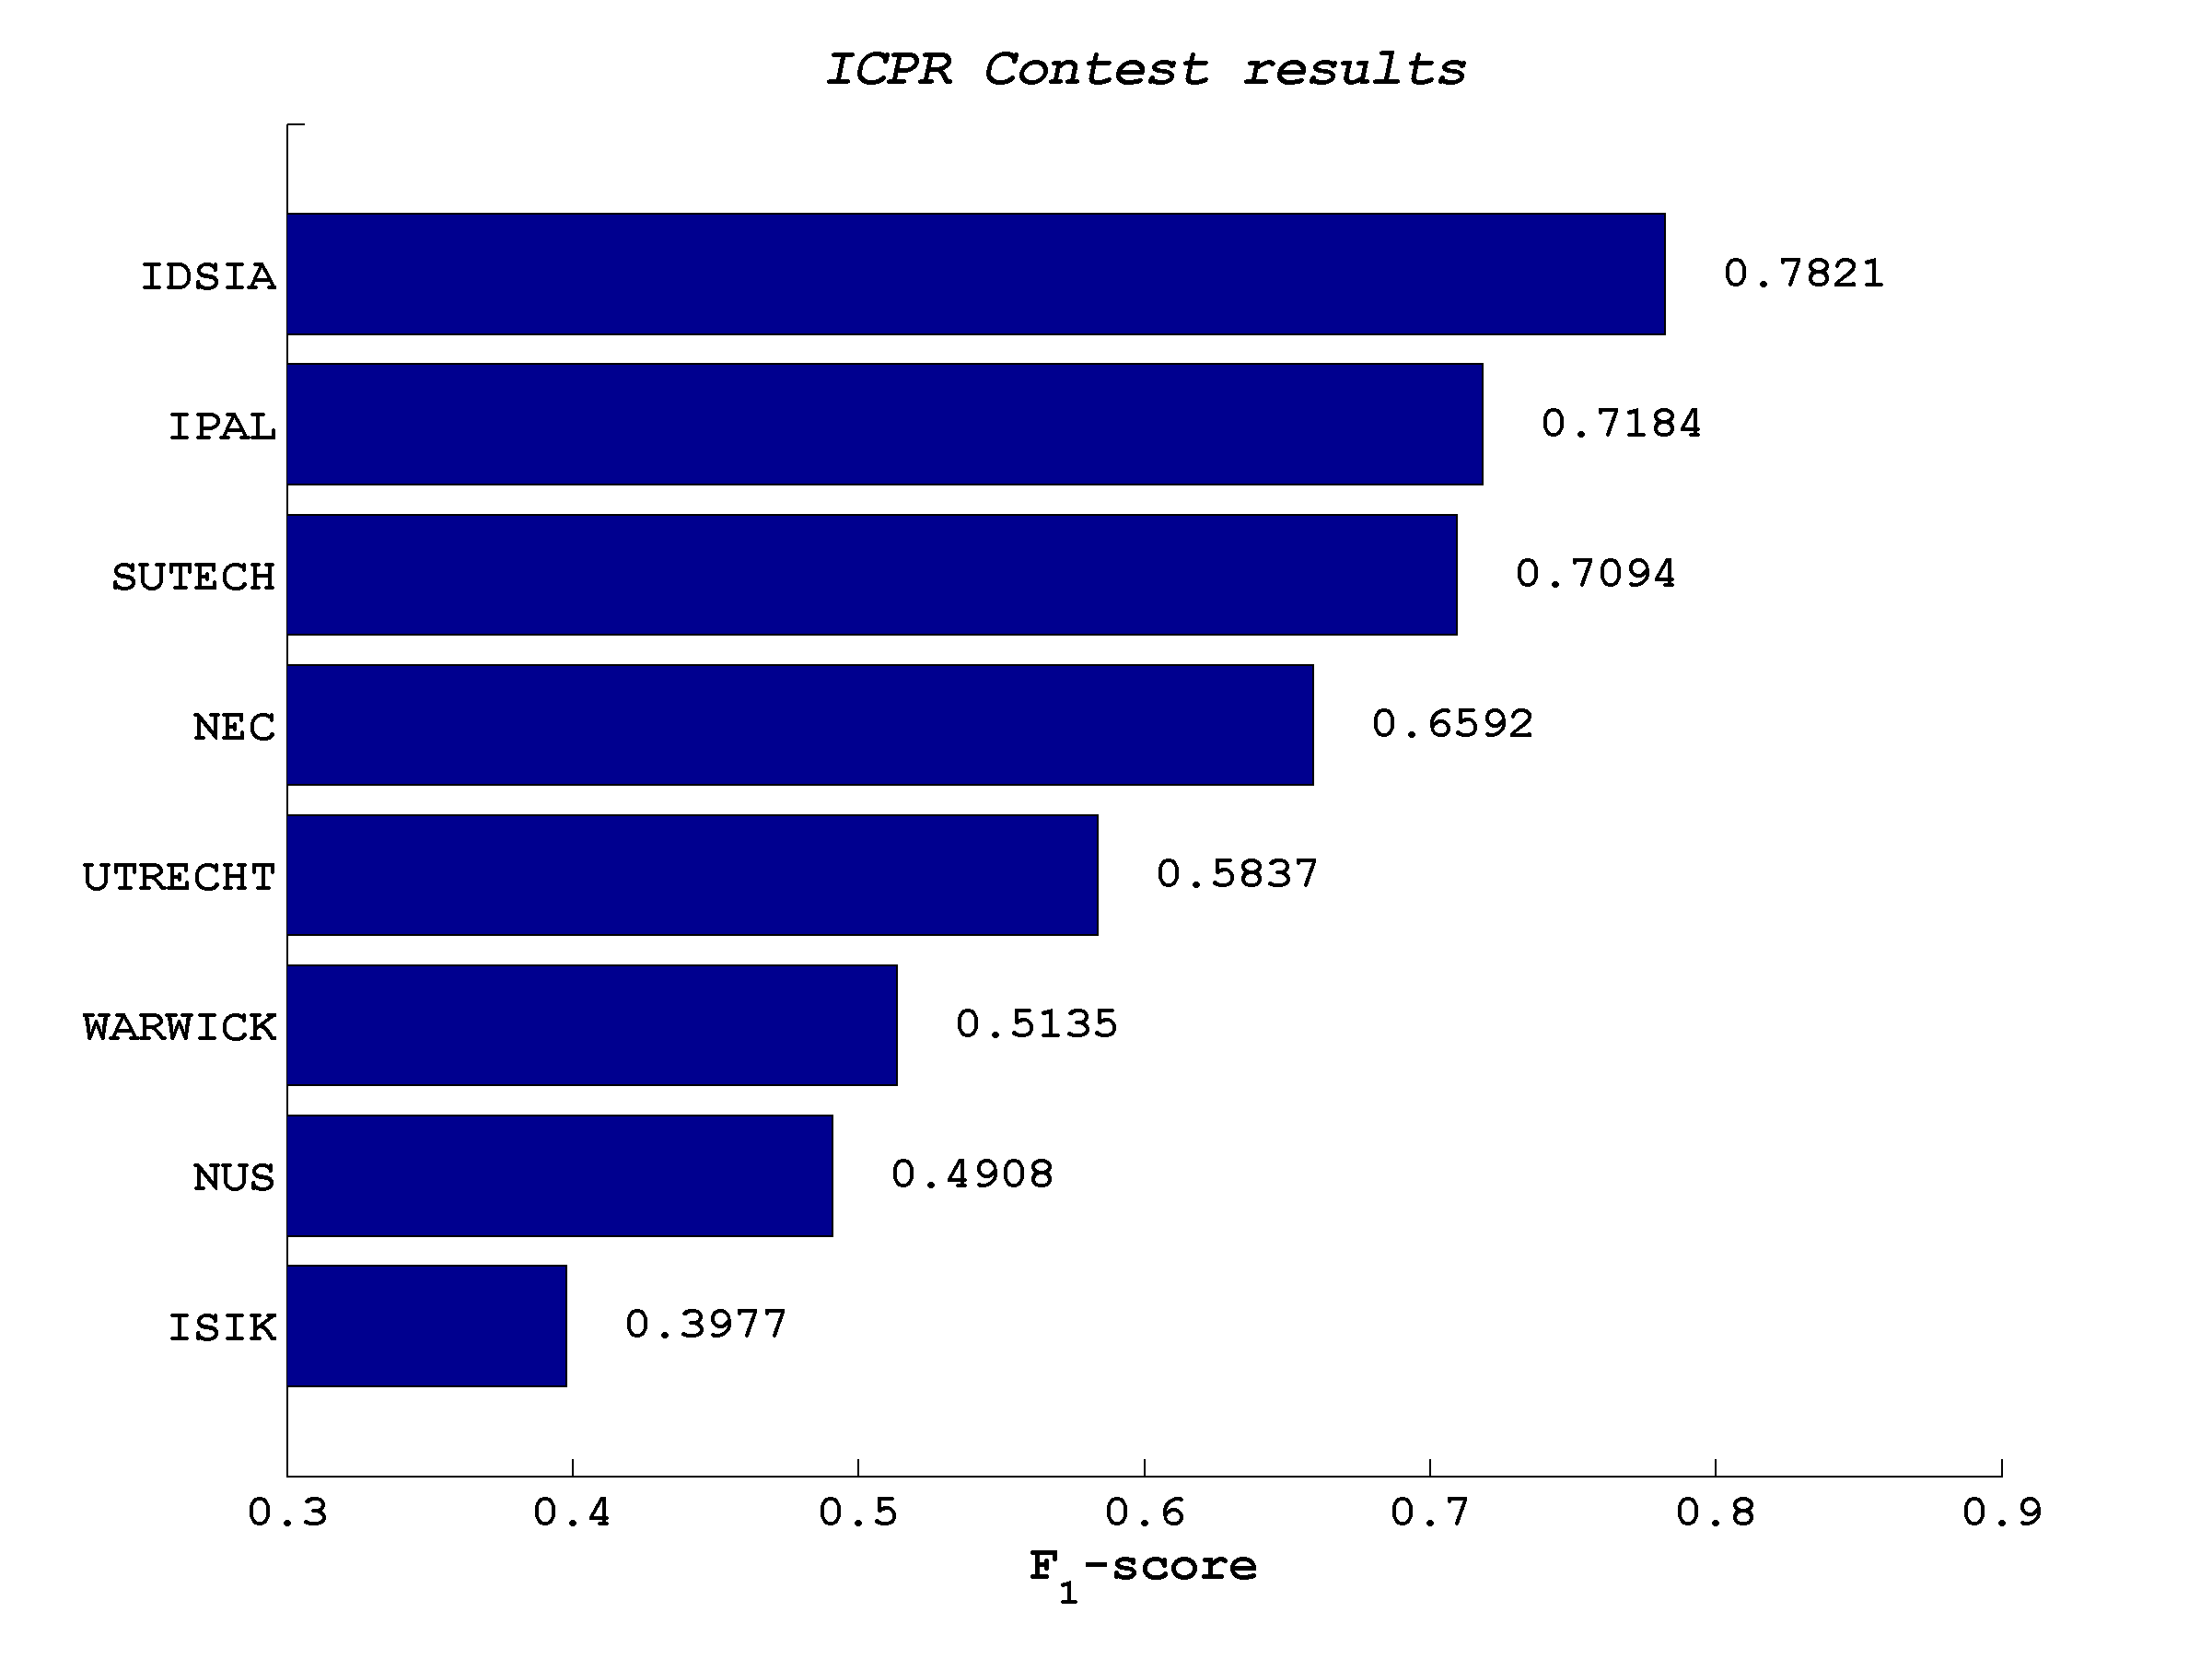
\includegraphics[width=0.82\textwidth]{./images/ICPRperf1.png}
      \label{ch6:fig3:a}
    }\\
    %\hspace{1mm}
    \subfigure[metrics]{
      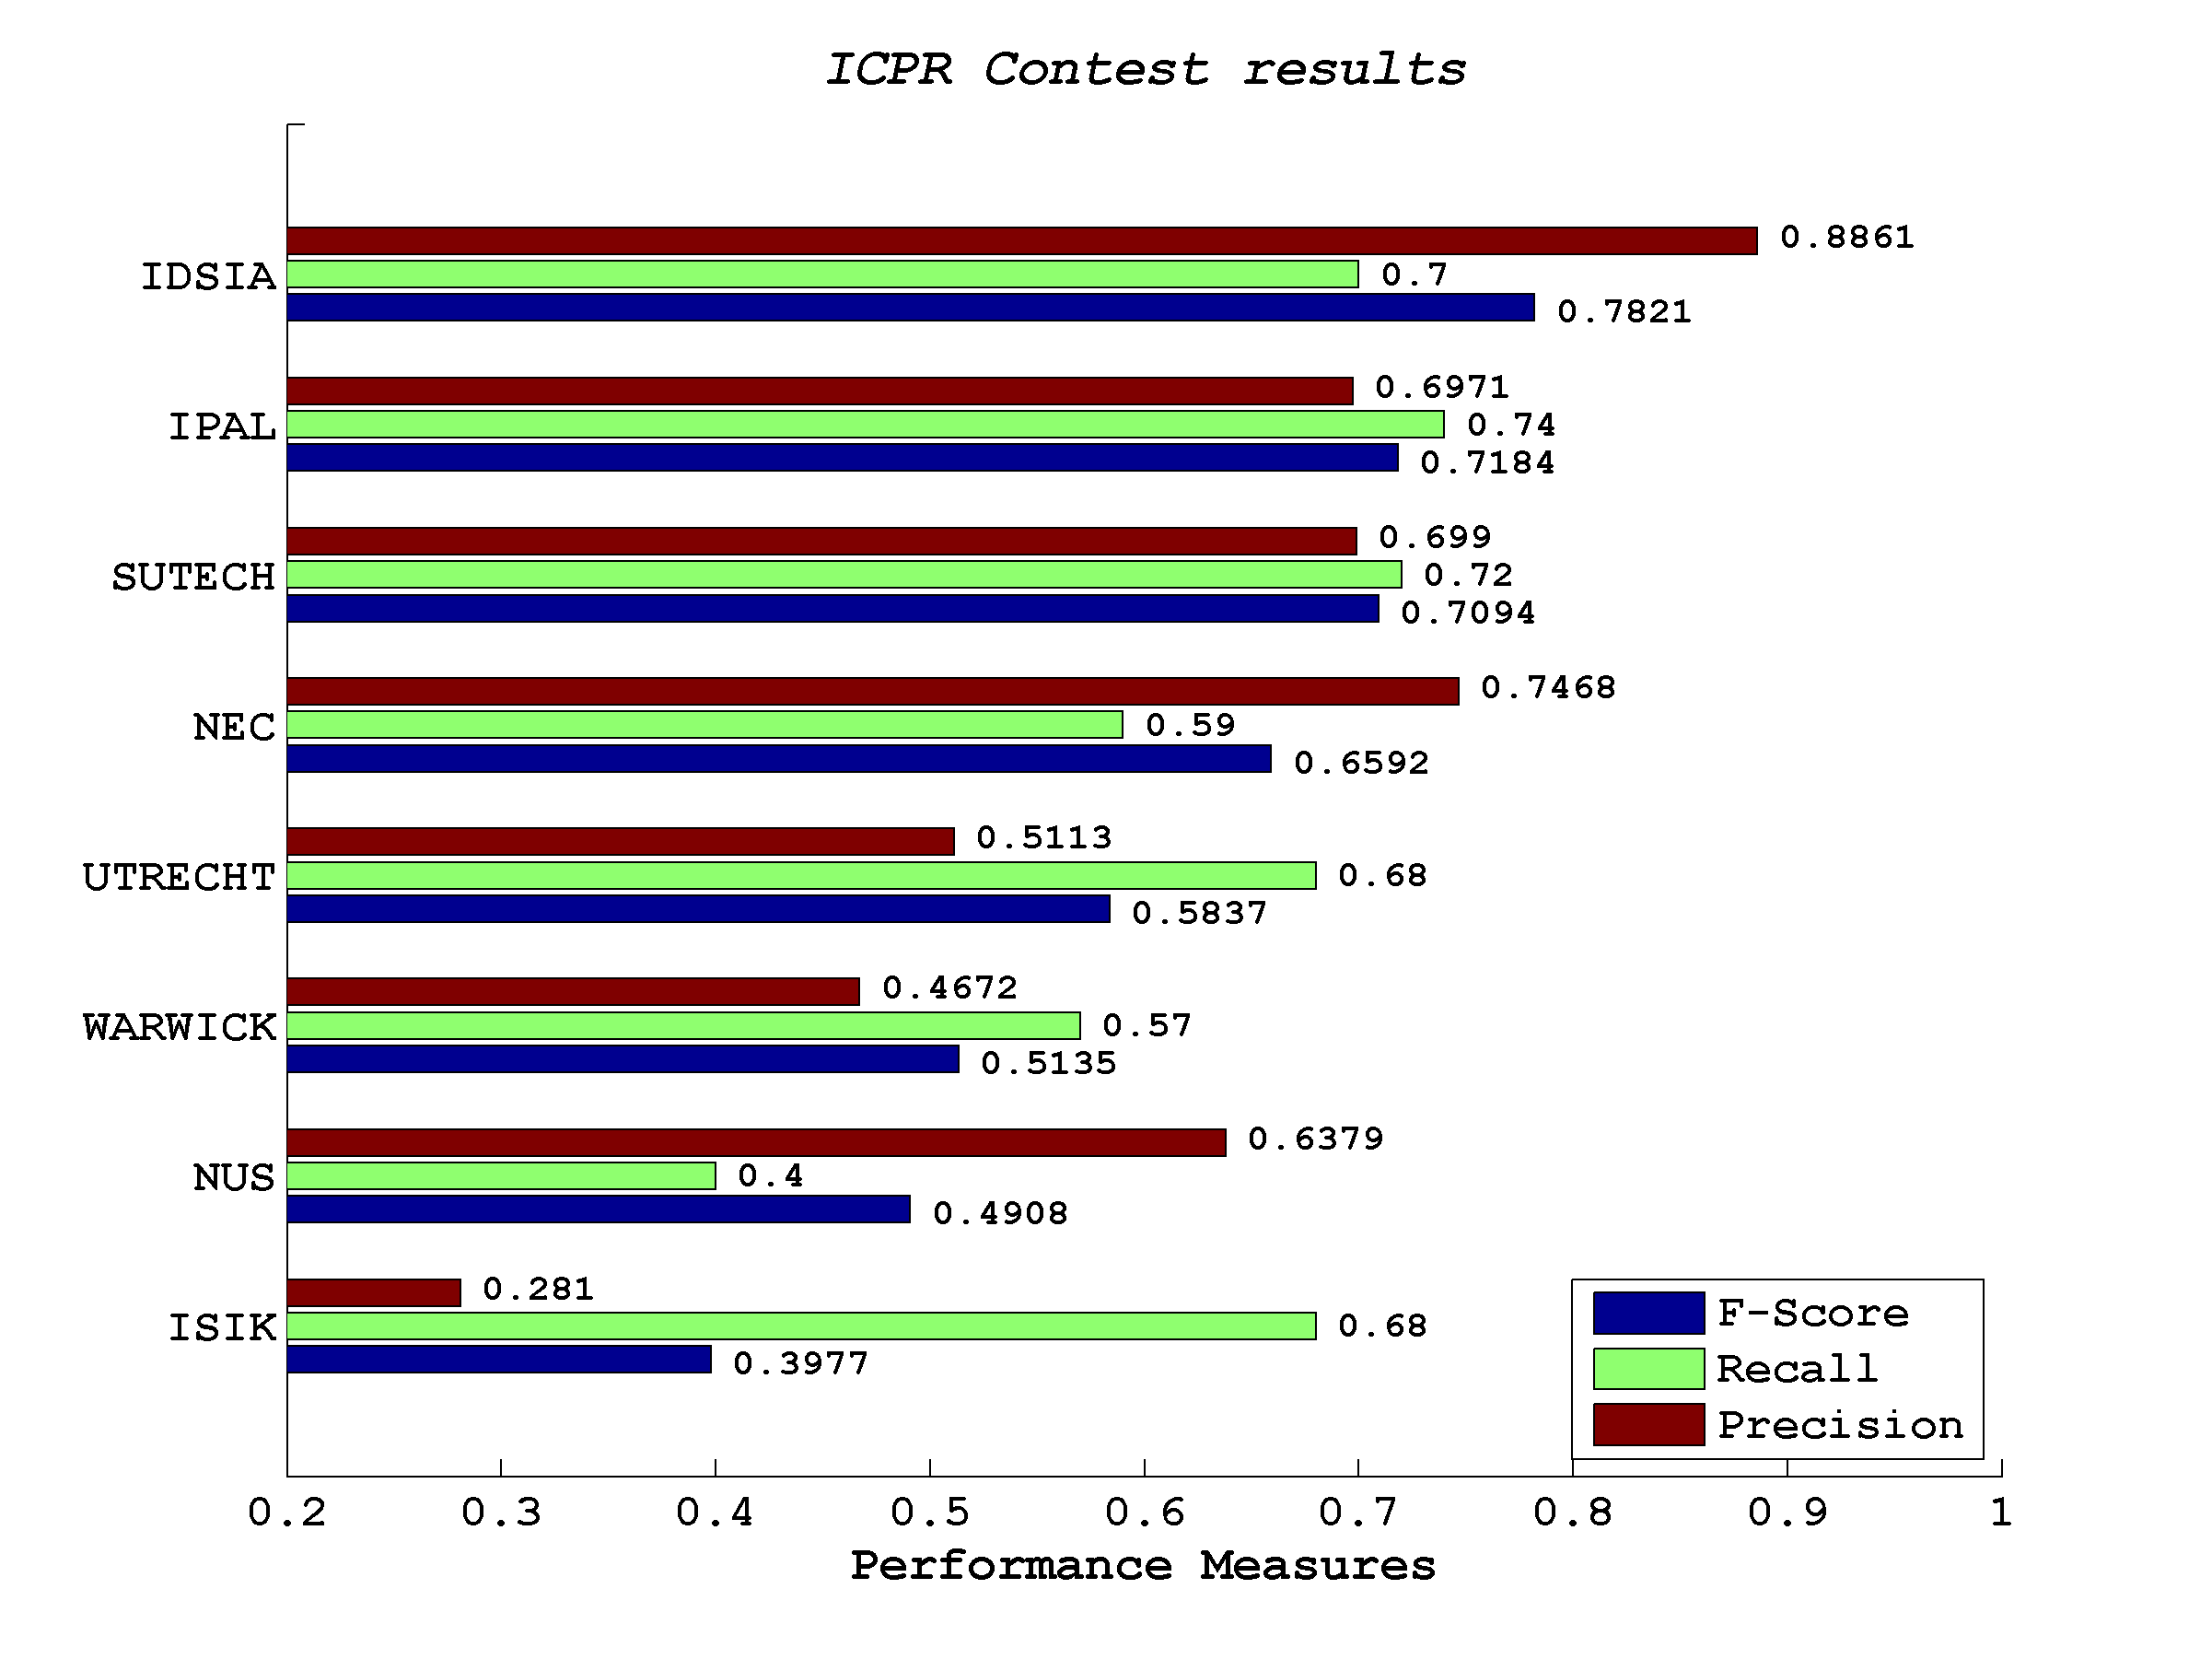
\includegraphics[width=0.82\textwidth]{./images/ICPRperf2.png}
      \label{ch6:fig3:b}
    }
    \caption{Performances of best algorithms in ICPR 2012 contest}
    \label{ch6:fig3}
\end{figure}